\newpage
\section{Mechanical engineering - Chloe}
\label{sec:me}

A connected plush toy is not a common engineering project. We achieved good results by collaborating closely with the ECAL designers, in particular Chloe and Marjane worked together on the plush toy, Soft PCB and blackbox design. \\
In addition to a "regular" project tasks such as designing a PCB and housing, we had to design a plush toy, and more importantly, soft electronics that would integrate inside the plush toy without being felt by the child. Designing electronics with textile comes with its own specific challenges, such as ensuring the flexibility of all components while avoiding short circuits from non-insulated "cable" threads or avoiding interferences in capacitive touch sensors.  

%\missingfigure[]{Illustration of all components/parts: Blackbox, Soft PCB, Plush toy, capacitive touch sensors}

\begin{figure}[ht]
    \centering
    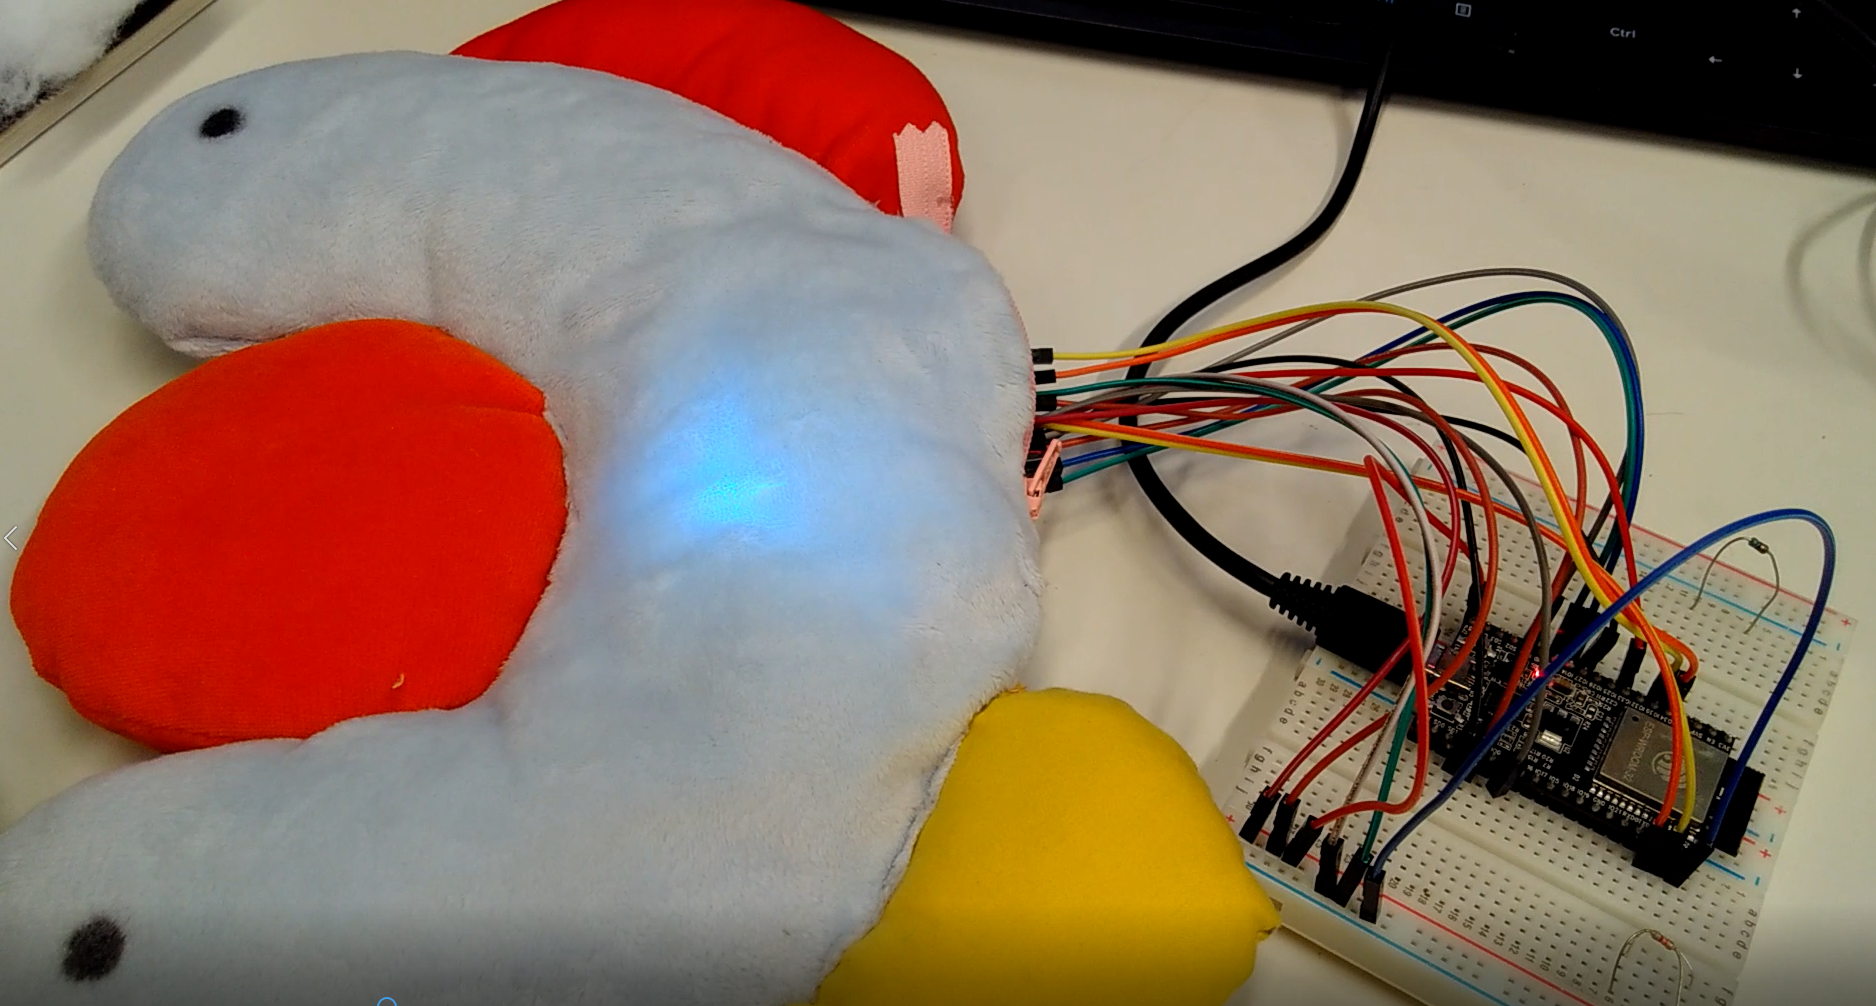
\includegraphics[width=0.8\textwidth]{images/HW/proto2_soft.PNG}
    \caption{Second prototype of our connected plush toy, as presented at MS5.}
    \label{fig:proto2}
\end{figure}

Terminology:
\begin{description}[align=left]
\item  [Blackbox] Inevitable "Hard" electronics such as microcontroller and battery, fitted in a slim housing inside of the plush toy.
\item [Soft PCB] Textile electronics for interactions, such as LEDs and capacitive touch sensors, designed with conductive textile and threads to be soft and "invisible" to touch inside of the plush toy 
\item [Skin] Soft textile layer surrounding all of the electronics, not taking into account any of the electronics components \ldots 
\end{description}

\subsection{Blackbox design}
The 3D modelling of the blackbox was carried on by Marjane as part of her industrial design tasks. However, we collaborated closely on brainstorming, defining shapes, connectivity and positioning of the blackbox in the prototype. 

\begin{figure}[ht]
    \centering
    \subfloat[3D rendering\label{fig:blackbox_3D}]{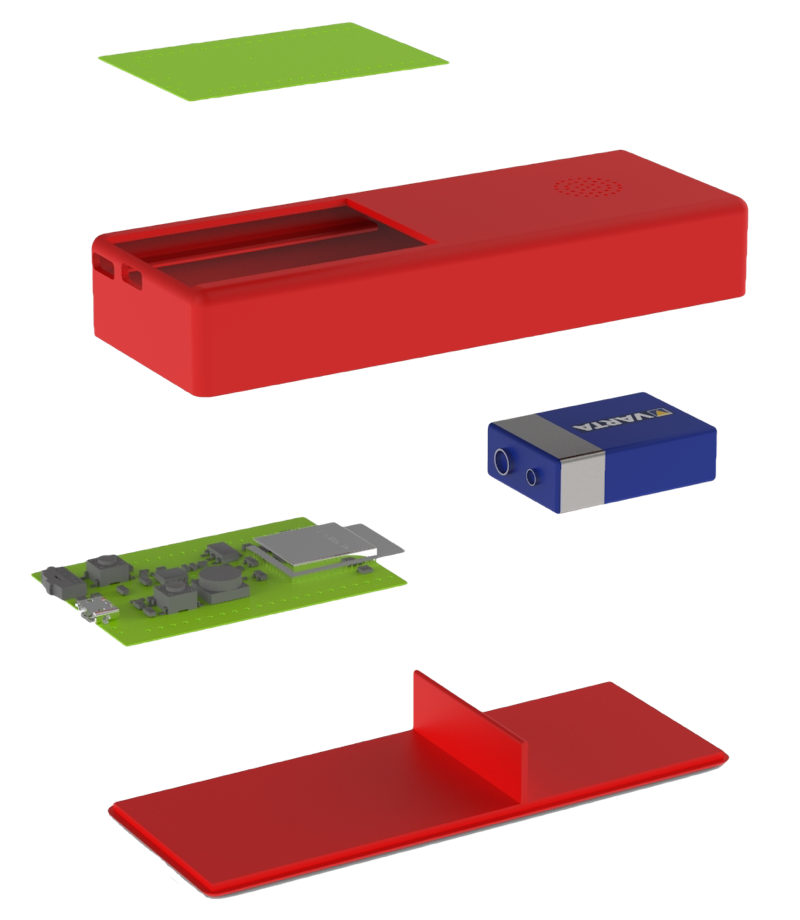
\includegraphics[width=0.35\textwidth]{images/HW/blackbox_v1.png}}\hfill
    \subfloat[3D printed blackbox with 3D printed PCB\label{fig:blackbox_v1}]{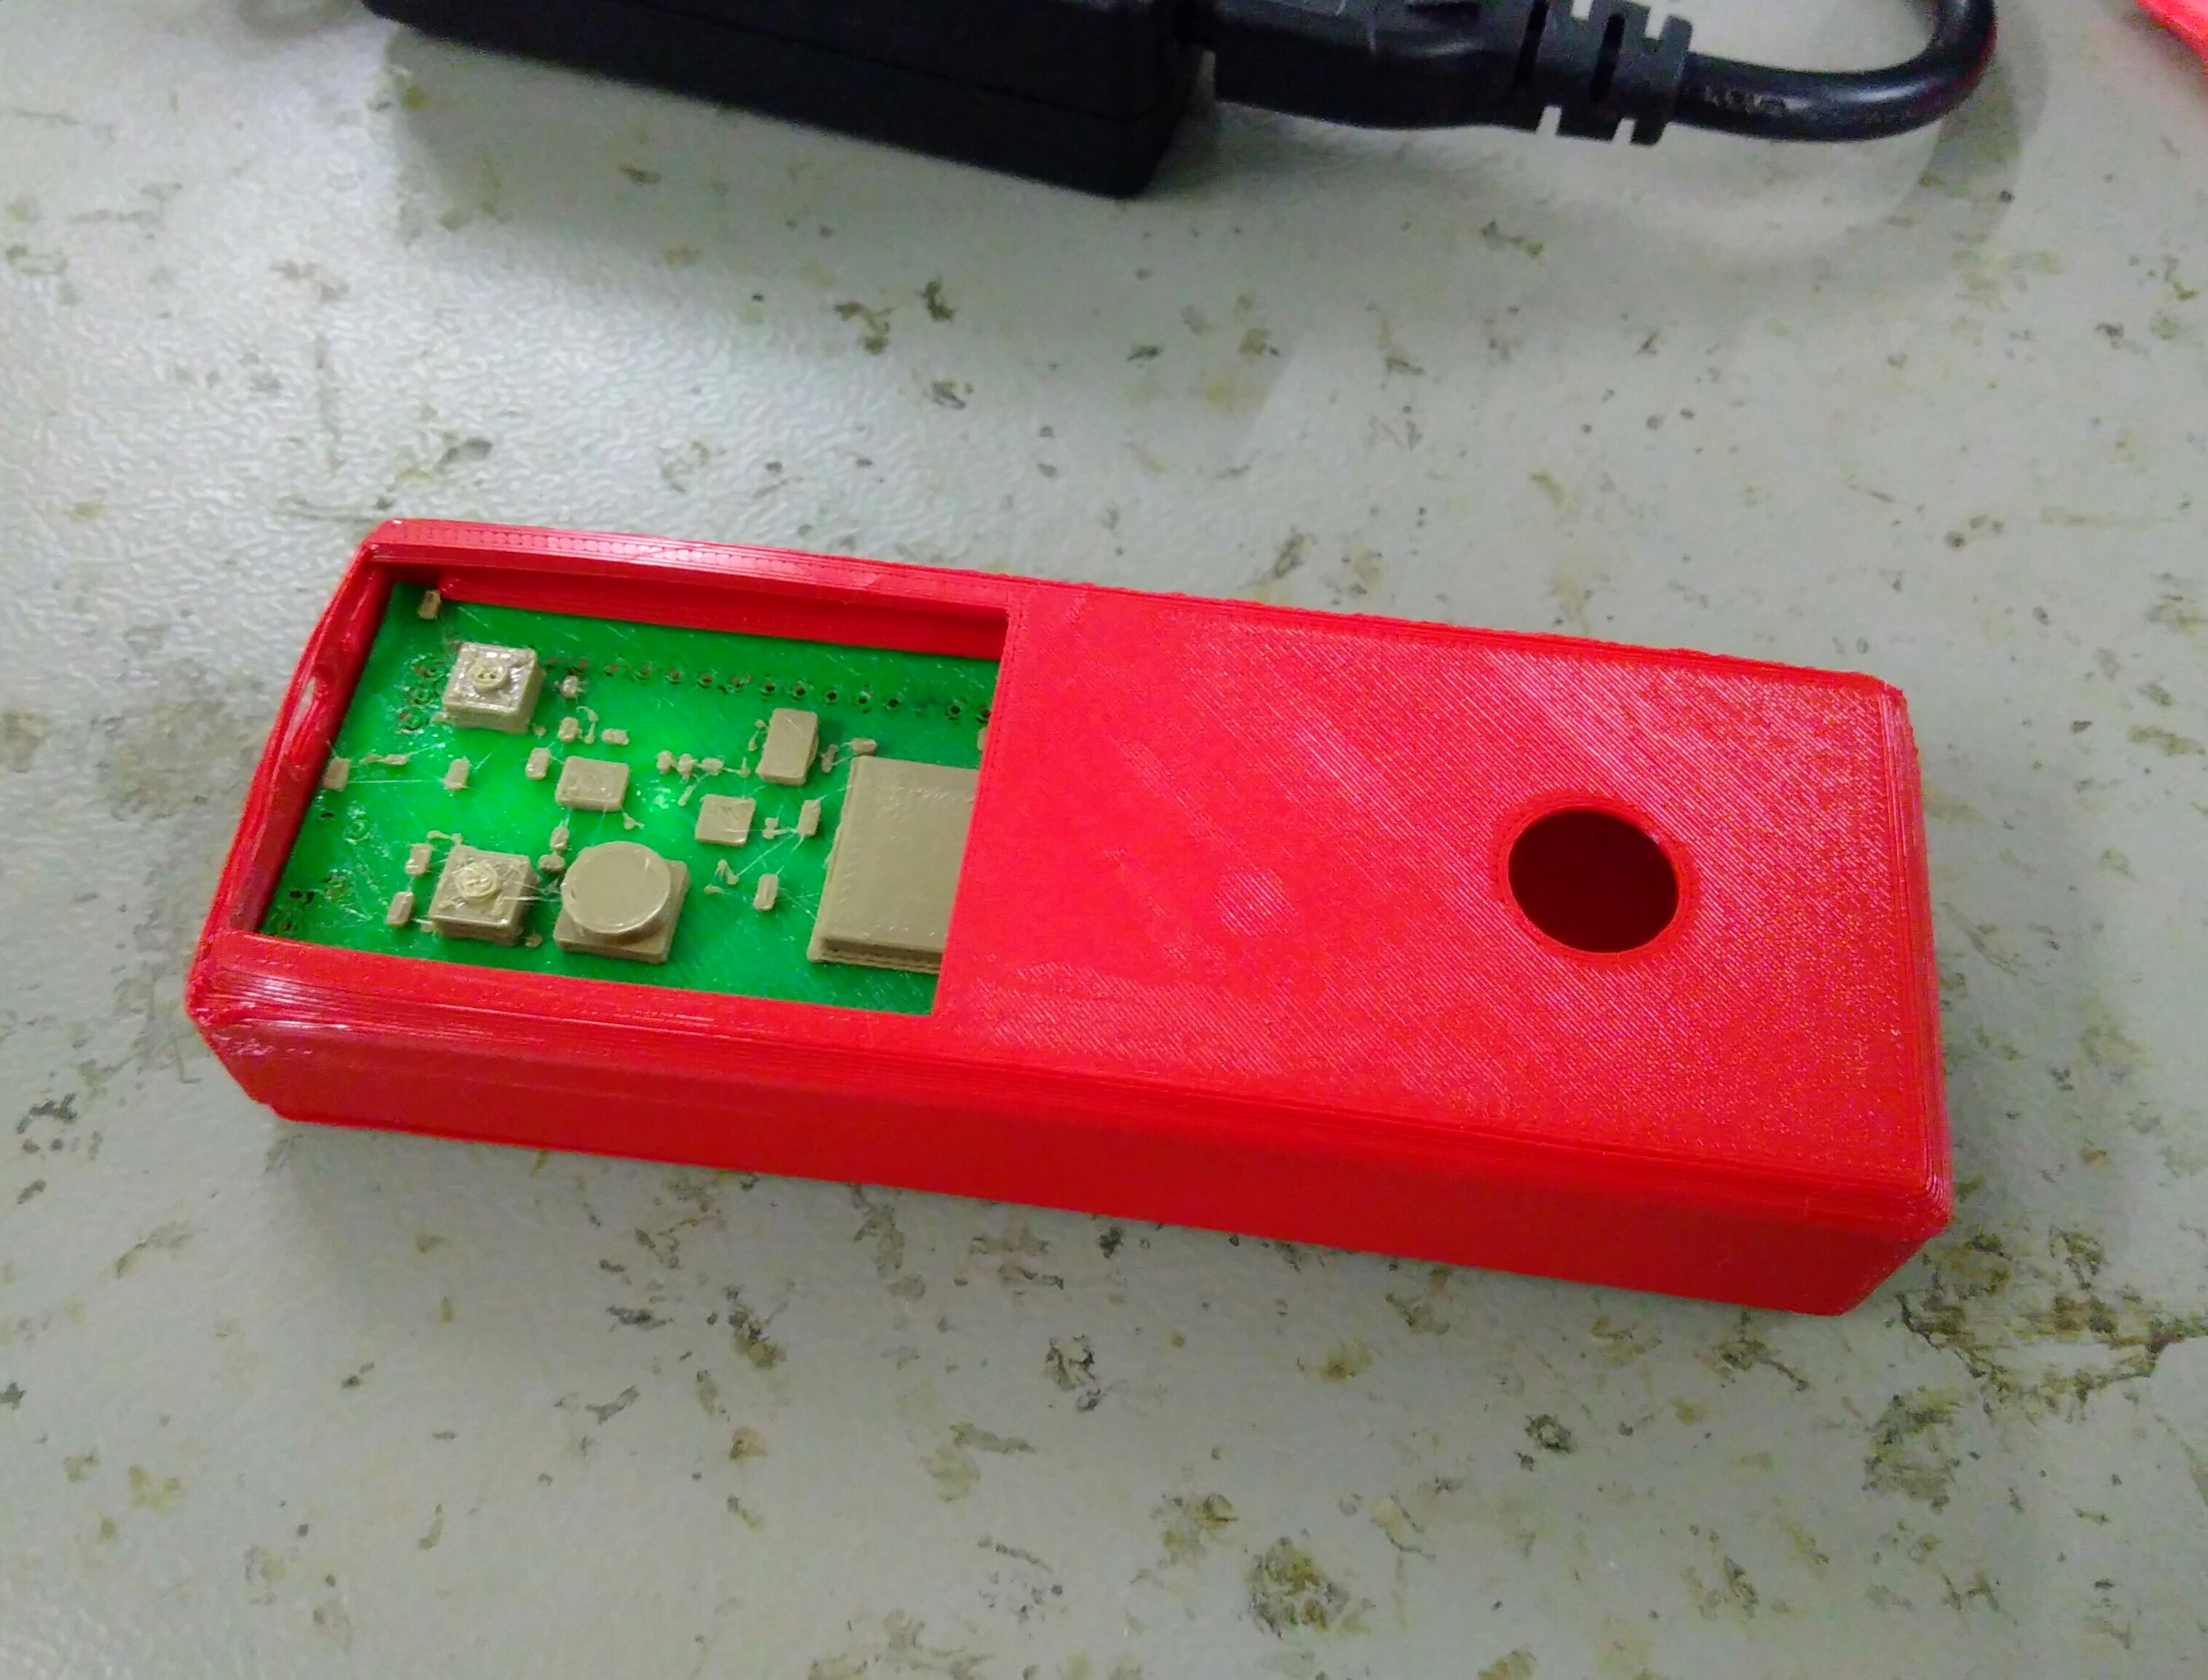
\includegraphics[width=0.6\textwidth]{images/HW/blackbox_3D.jpg}}\hfill
    \caption{First iteration of the blackbox design, including PCB, battery and loudspeaker}
    \label{fig:blackbox}
\end{figure}

\paragraph{Blackbox description} The blackbox holds the PCB, battery and speaker. It connects
to the Soft PCB through a secondary PCB breaking out the pin connections into textile conductors. The blackbox should be easily removable by the caretaker, give easy access to the battery for replacement/recharging and be easy to connect to the the soft PCB. In our current version, the blackbox is connected to the soft pcb through pins; in a future version a more user-friendly connector will be considered.

\paragraph{Textile considerations}
The blackbox has to fit inside of a plush toy and be as little intrusive as possible. We decided to make the blackbox in a rounded, elongated ("banana") shape following the curves of the plush toy. A pocket accessible through a zipper is designed to hold the blackbox and define the connections with the "soft PCB".

\begin{figure}[ht]
    \centering
    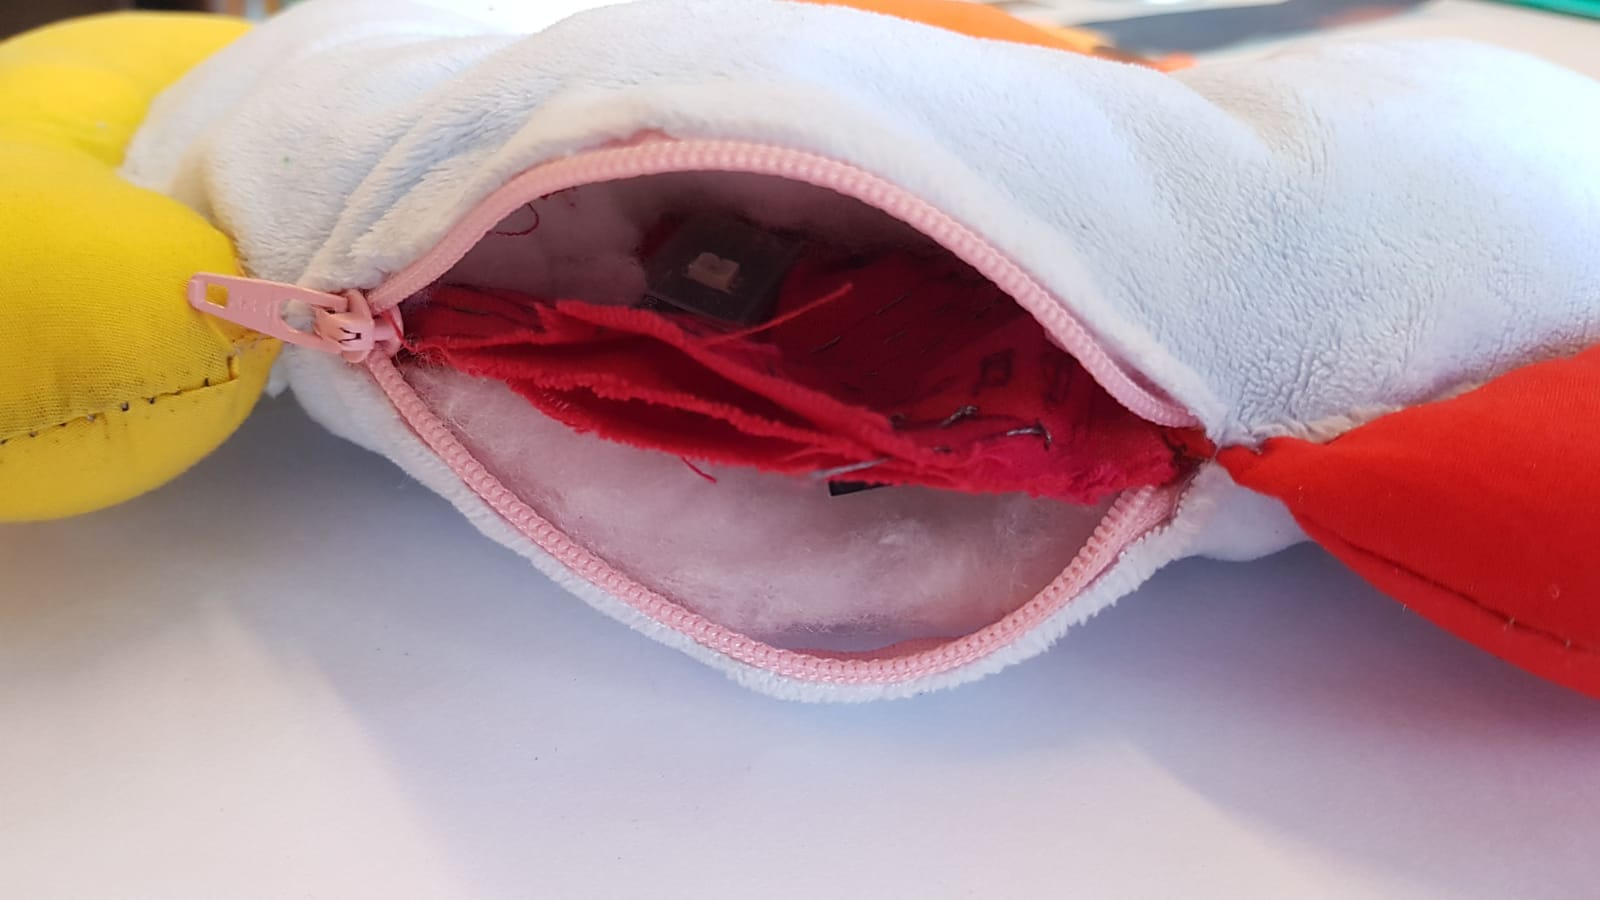
\includegraphics[width=0.6\textwidth]{images/HW/proto2_layers.jpg}
    \caption{Layers of the first prototype: outer skin, plush stuffing and soft PCB}
    \label{fig:heat_tracks}
\end{figure}

    \paragraph{PCB design}
In our current version of the PCB (iteration 1), we decided to break out the circuit with many pins to keep prototyping options open for connectivity of hard to soft interfaces. The main PCB is linked to the Soft PCB through a secondary hard PCB, attached to the textile, to which conductive threads are tied, linking the elements (LED, sensors).
    
To achieve the smallest possible form factor, we decided to re-desing the shape of the PCB for a future version according to the desired shape of the blackbox. For this, we take into consideration the hard/soft connections, buttons, positioning of connectors, battery and speaker elements. 

\subsection{Soft PCB} The "Soft PCB" is a 3-layer 2D fabric "PCB" with a first layer of textile and conductive touch pads, an insulating layer and a second textile layer with LEDs and conductive thread or textile conductor tracks linking the LEDs. The tracks are connected to pins in the current version of the prototype and will be linked to the secondary PCB in the next iteration of the prototype. In a future iteration of the prototype, we will consider a more compact, robust and user-friendly connector.


\begin{figure}[H]
    \centering
    \subfloat[Textile capacitive sensors on soft PCB\label{fig:soft_capa}]{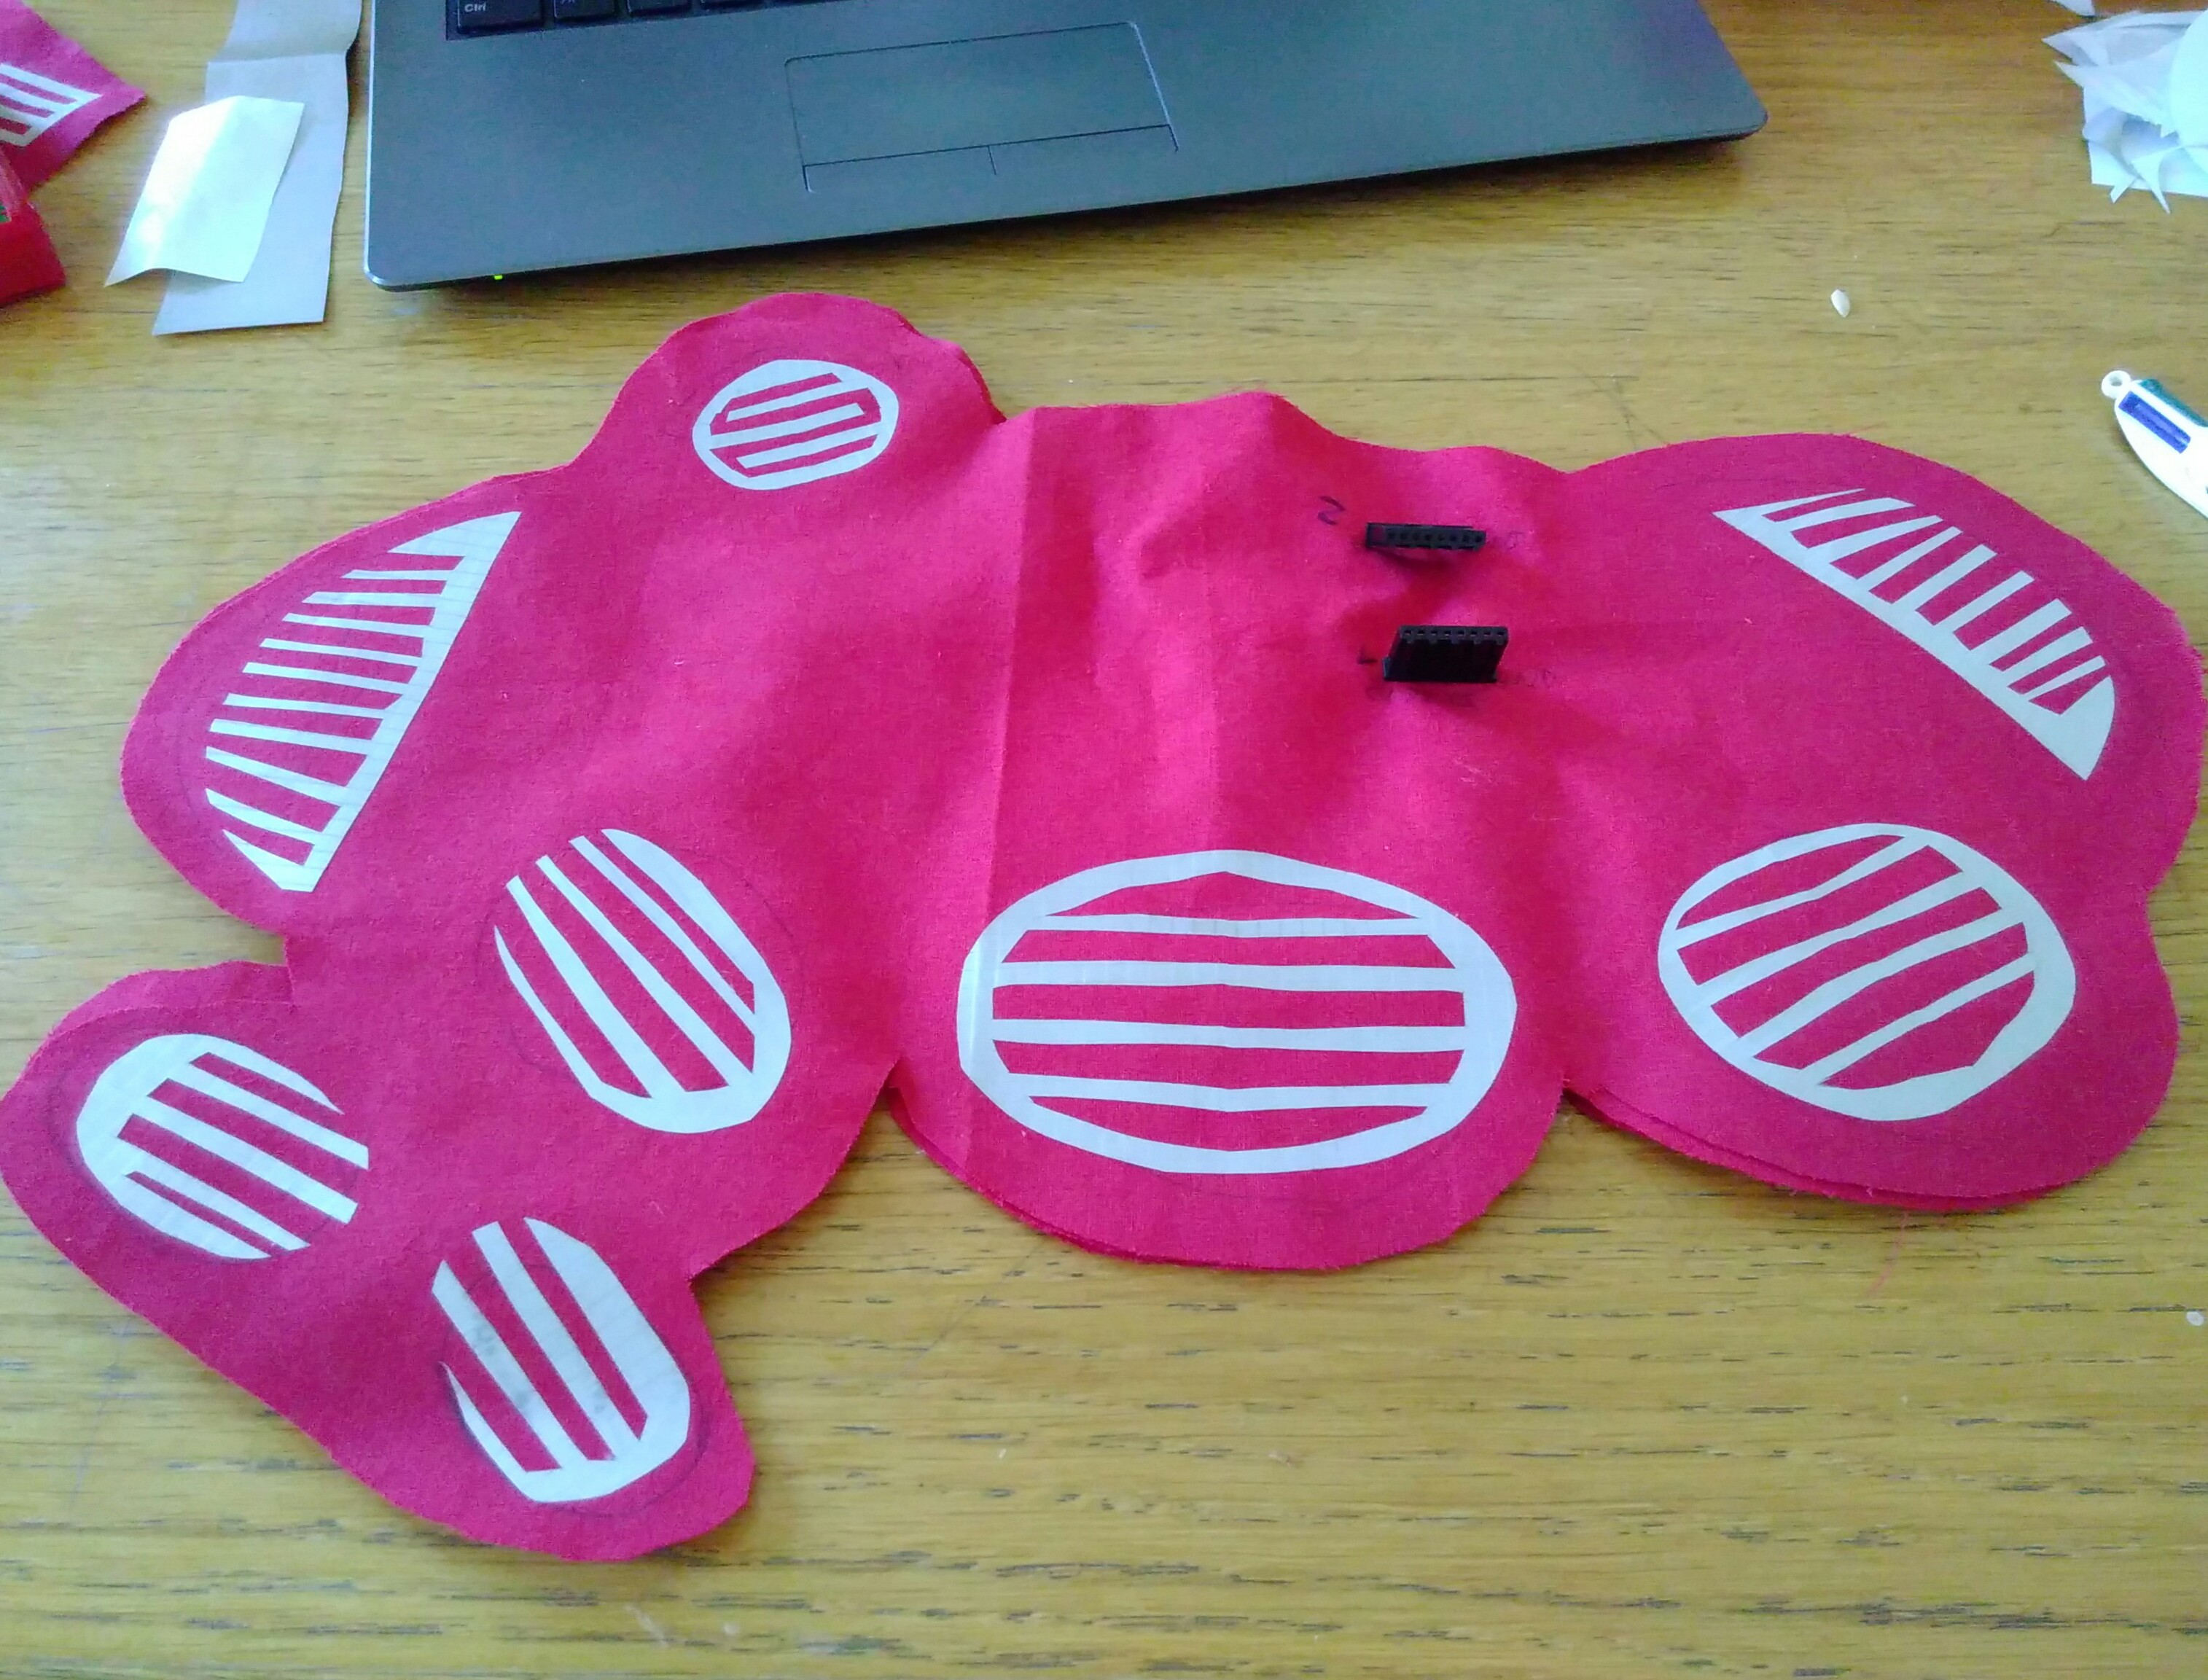
\includegraphics[width=0.47\textwidth]{images/HW/softPCB_sensors2.jpg}}\hfill
    \subfloat[Conductive thread linking the LEDs\label{fig:soft_threads}] {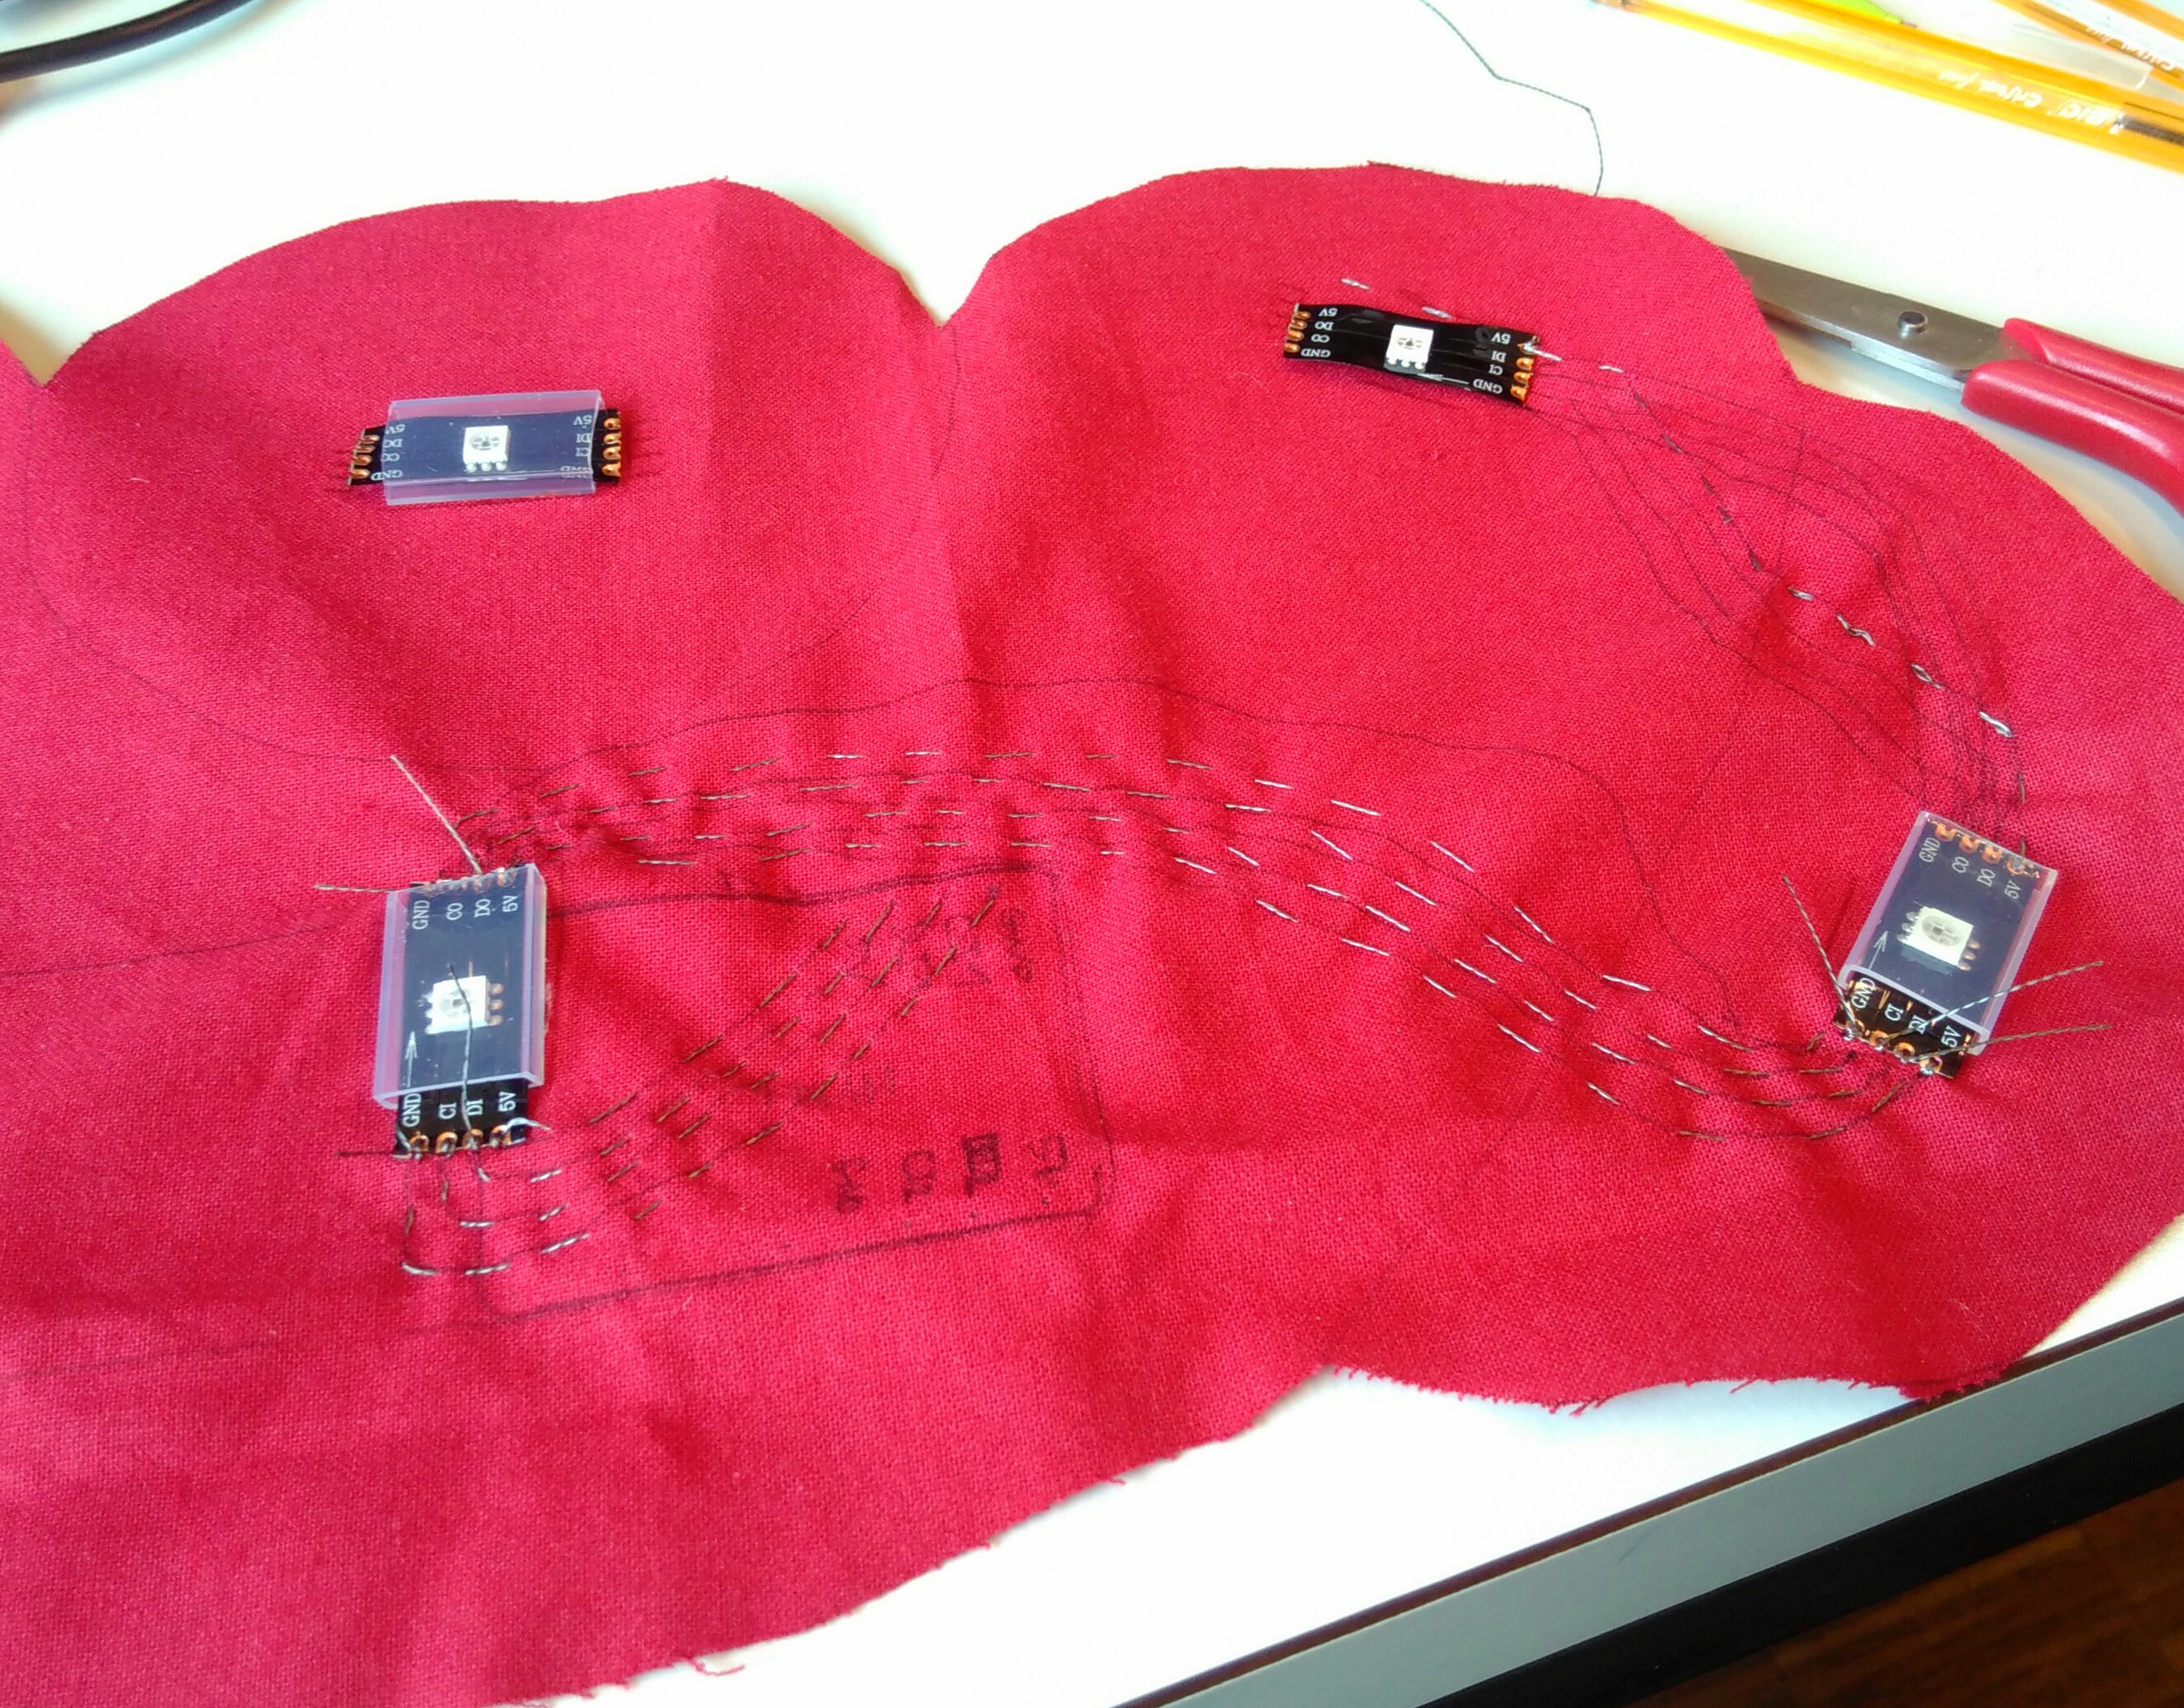
\includegraphics[width=0.47\textwidth]{images/HW/softPCB_LED_thread.jpg}}\hfill
    \caption{Details of top and lower layers of soft PCB} 
    \label{fig:soft_pcb}
\end{figure}

\subsubsection{Washability} Our goal for the plush toy would be to be fully machine-washable once the blackbox is removed. The electronics (LEDs, connectors) would ideally be sealed in silicon while the textiles can endure a small number of washing cycles.

\subsubsection{Manufacturing options} For the first two prototypes, the LEDs were hand sewn to the soft PCB. The touch sensor pads were either machine sewn or heat-bonded to the textile support. As it is, the soft PCB takes several hours of tedious handwork to manufacture. We are currently experimenting with using the heat-bond conductive fabric on both sides of the soft PCB on which LEDs will be directly soldered (Fig. \ref{fig:heat_tracks}). 

\begin{figure}[ht]
    \centering
    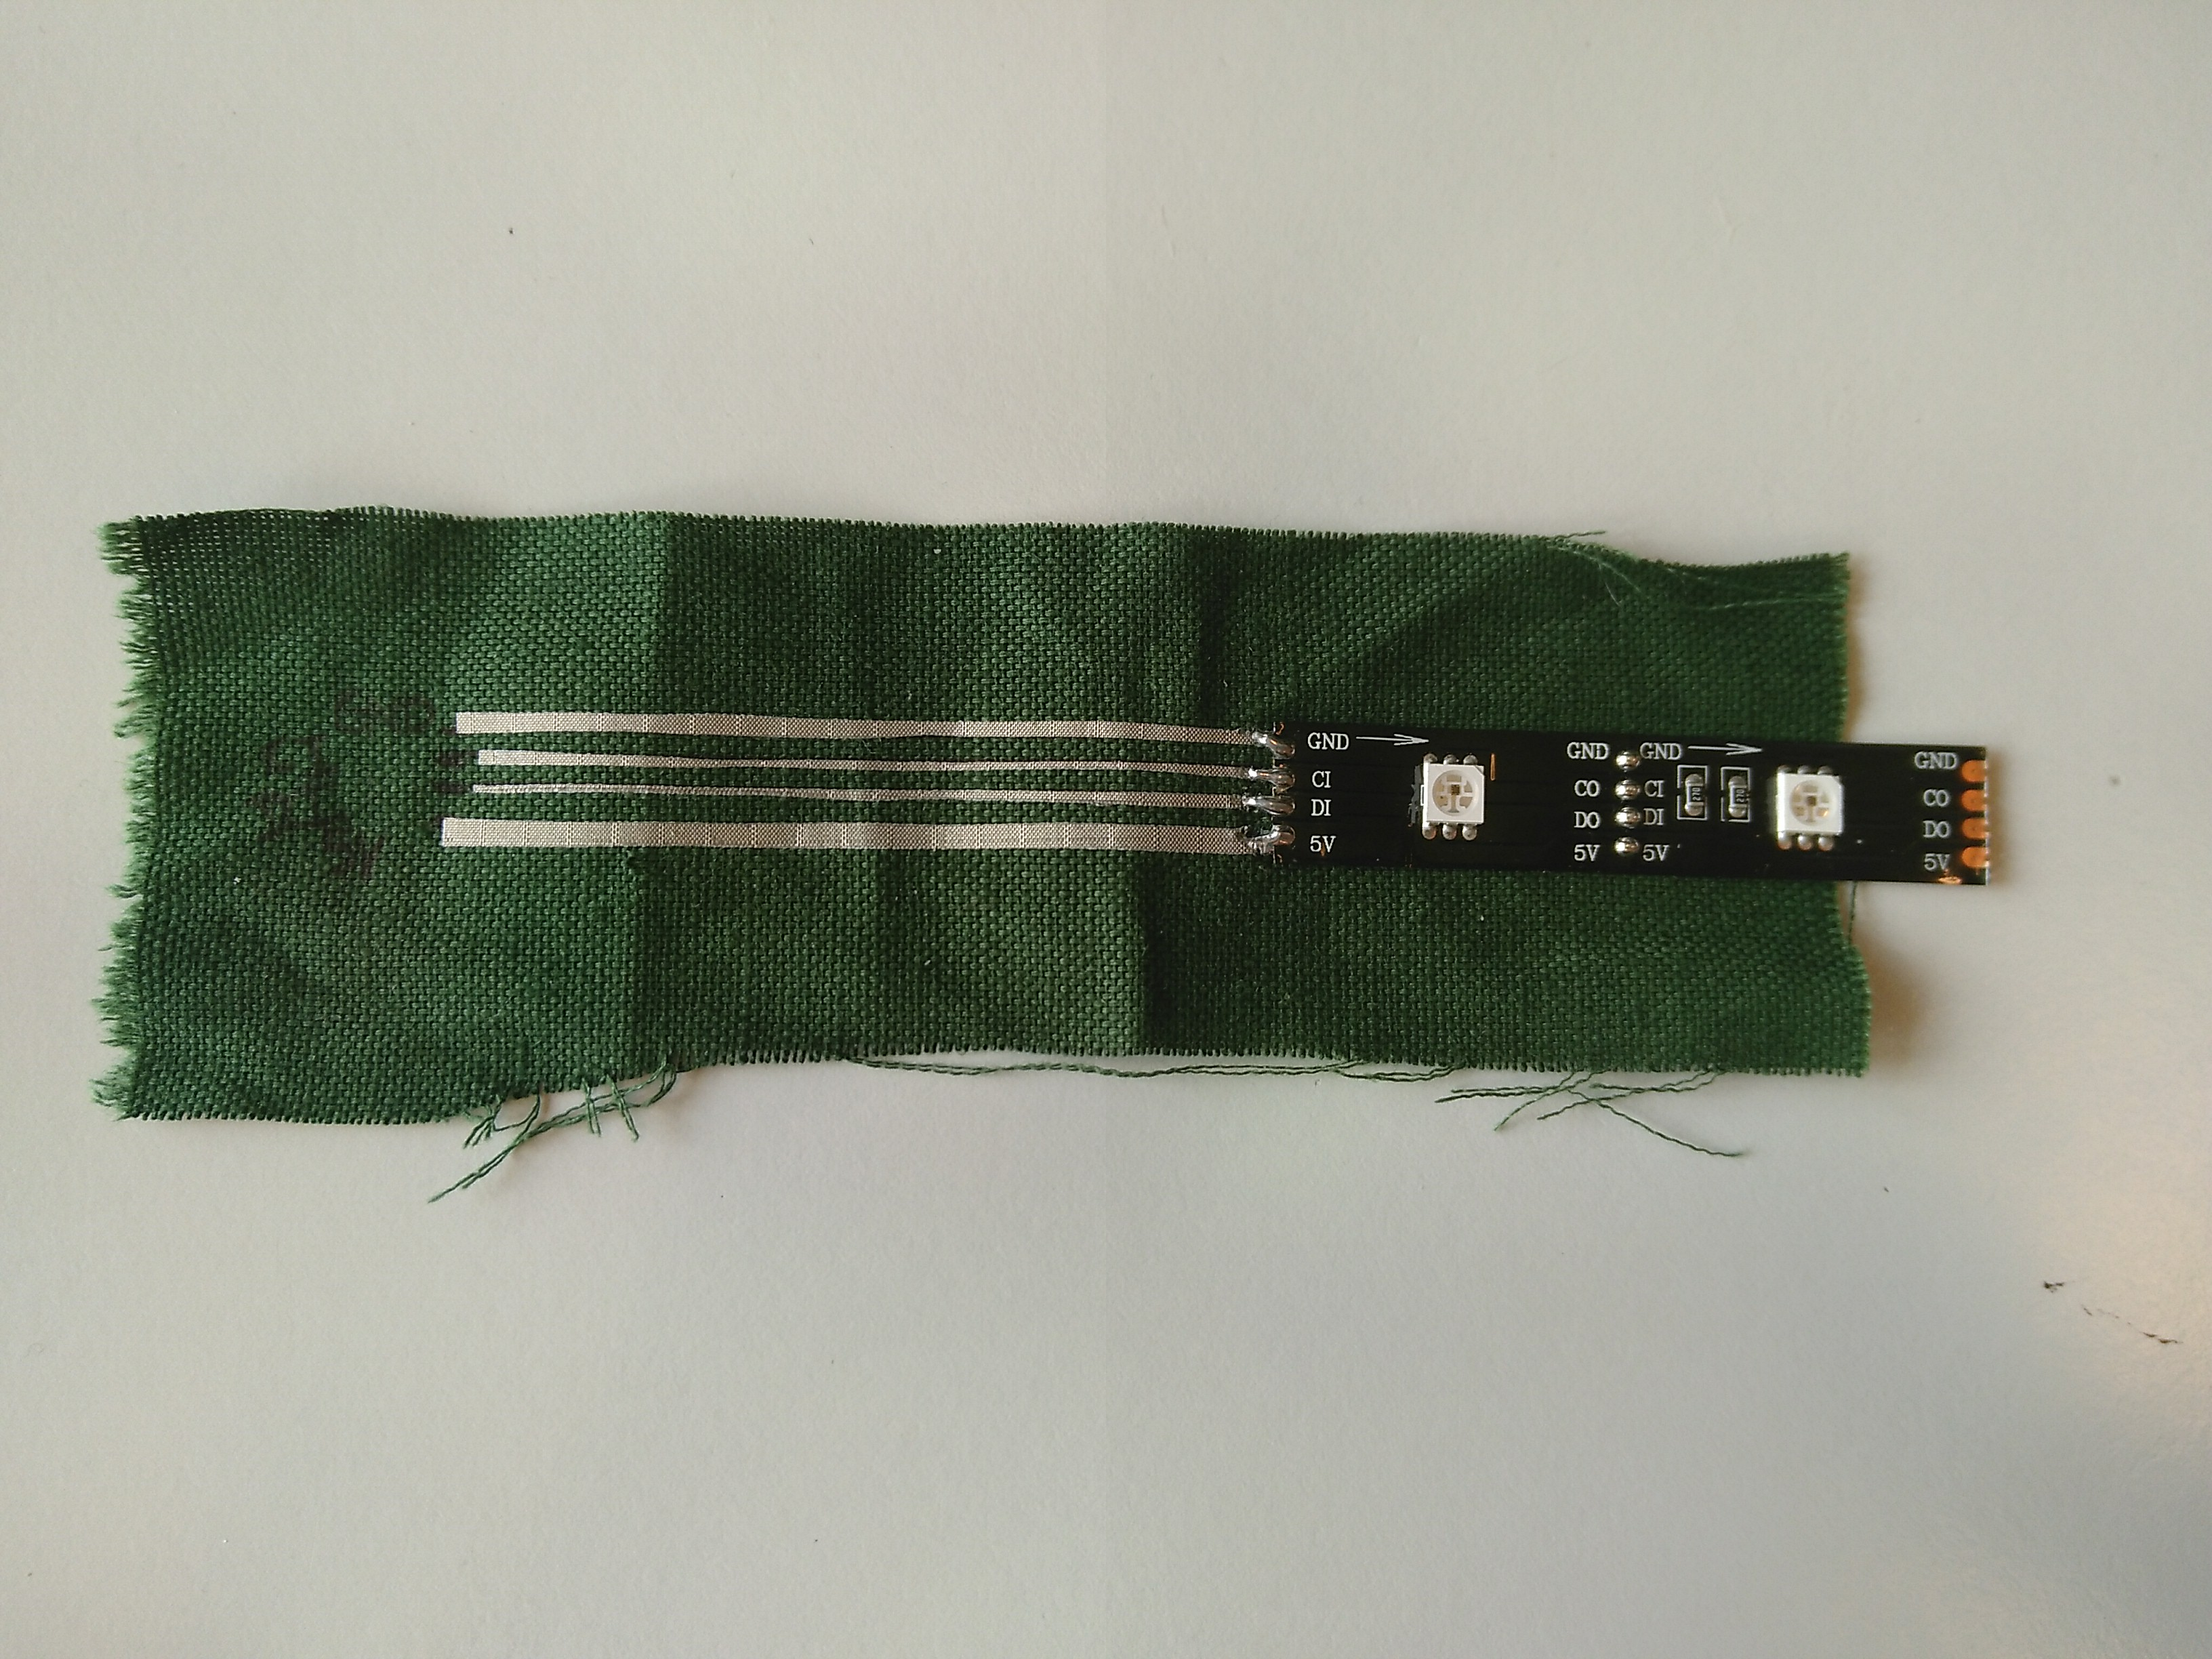
\includegraphics[width=0.6\textwidth]{images/HW/heatbond_tracks.jpg}
    \caption{Test sample of heat-bonded conductive tracks}
    \label{fig:heat_tracks}
\end{figure}

\subsection{Soft sensors}
    \subsubsection{ESP32 integrated capacitive touch sensors}
In our project, we take advantage of the ESP32's integrated capacitive touch sensors. These are linked to conductive textile pads on the Soft PCB. 

\begin{figure}[ht]
    \centering
    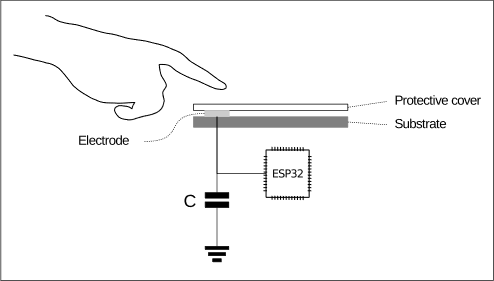
\includegraphics[scale=0.5]{images/FW/esp_touchsensor.PNG}
    \caption{ESP32 built-in touch sensor}
    \label{fig:esp_touchsens}
\end{figure}

    \subsubsection{Prototyping design}
For our prototypes, we have experimented with different test codes, different materials and different touch pad designs.

\paragraph{Conductive materials} We experimented with conductive knit and woven textile from Adafruit, conductive paint from Bare Conductive and heat-bond conductive fabric from Less EMF. The latter is the best in terms of manufacturability as it can easily be attached to the soft PCB fabric and is less susceptible to fraying and creating short circuits. The conductive paint is great for prototyping and fixing small connectivity issues but is water-soluble so it will not be considered as a reliable maufacturing option for the prototype (if sealed in acrylic it may be considered, especially for manufacturing speed such as in silk-screen printing). 
    \subsubsection{Experimenting with soft sensors} 
We experimented several types of soft sensors and materials: bend sensors with Velostat; stretch and pressure sensors with Eontex and a potentiometer thread from Adafruit. After considering manufacturability, ease of integration, repeatability, interaction possibilities and costs, we decided to keep only the touch/press sensors.

\begin{figure}[H]
    \centering
    \subfloat[Velostat bend sensor\label{fig:softsens_bend}]{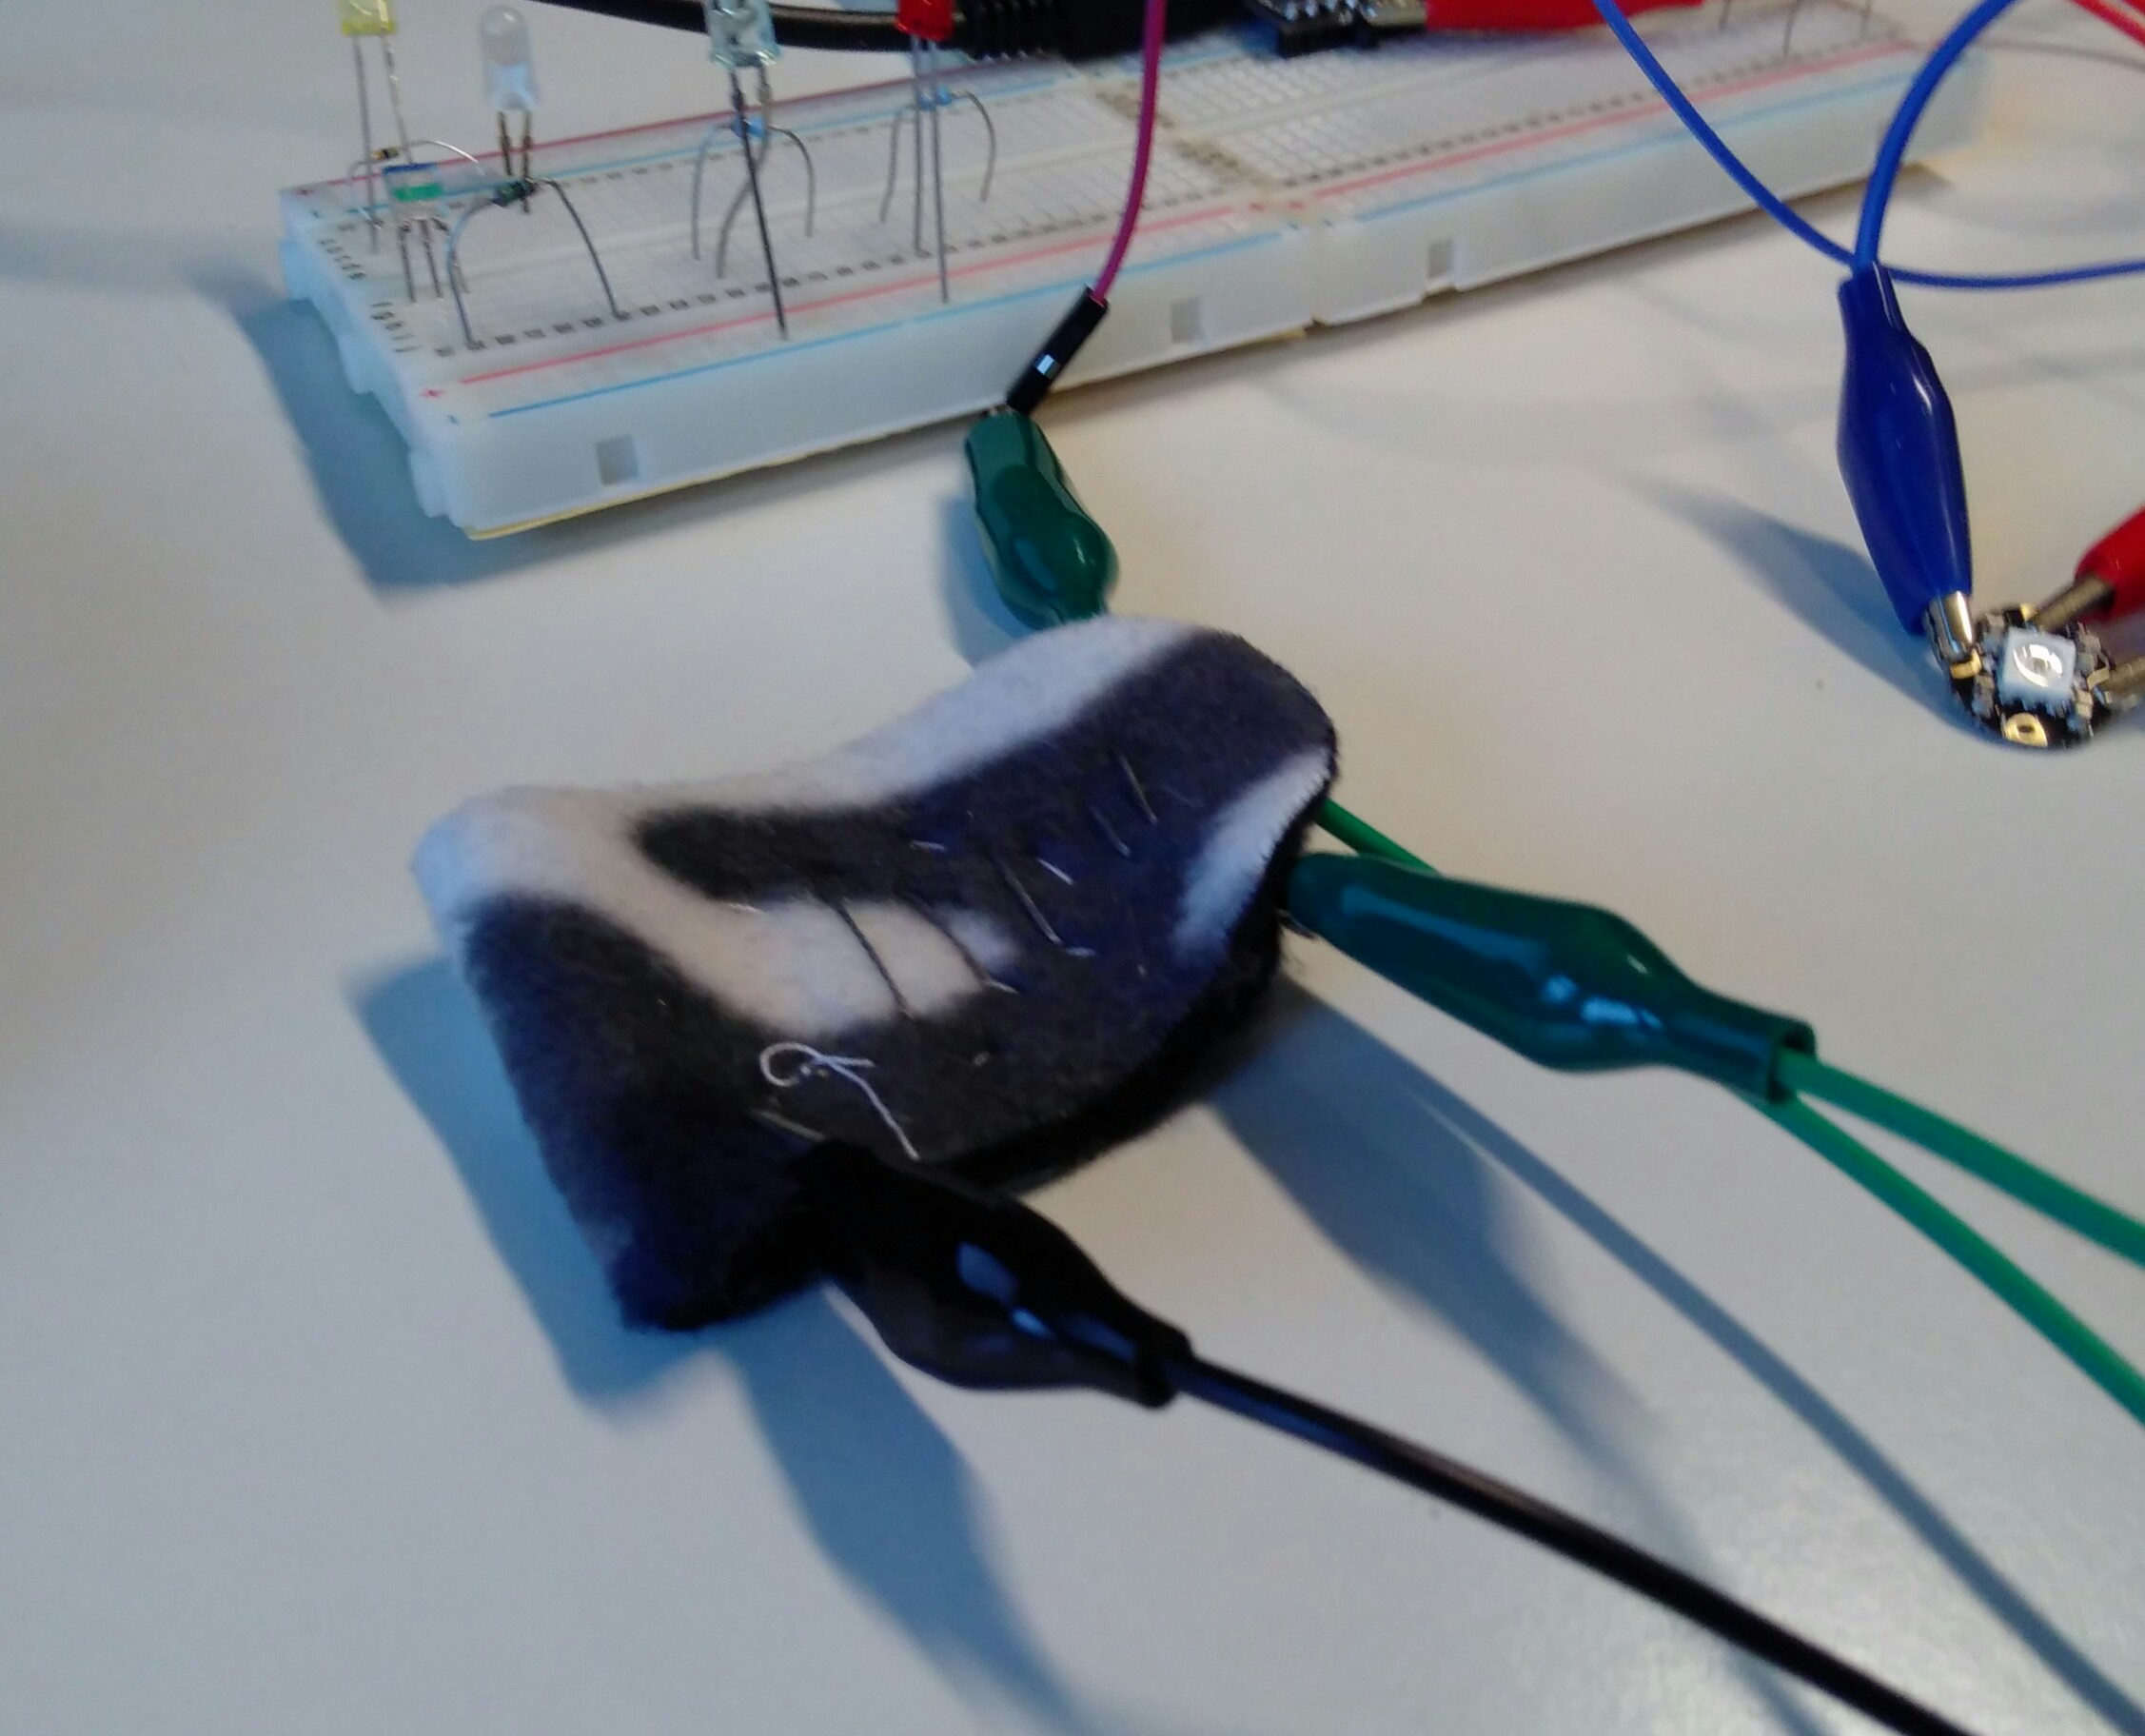
\includegraphics[width=0.47\textwidth]{images/HW/softsens_bend.jpg}}\hfill
    \subfloat[Eontex stretch sensor\label{fig:softsens_stretch}] {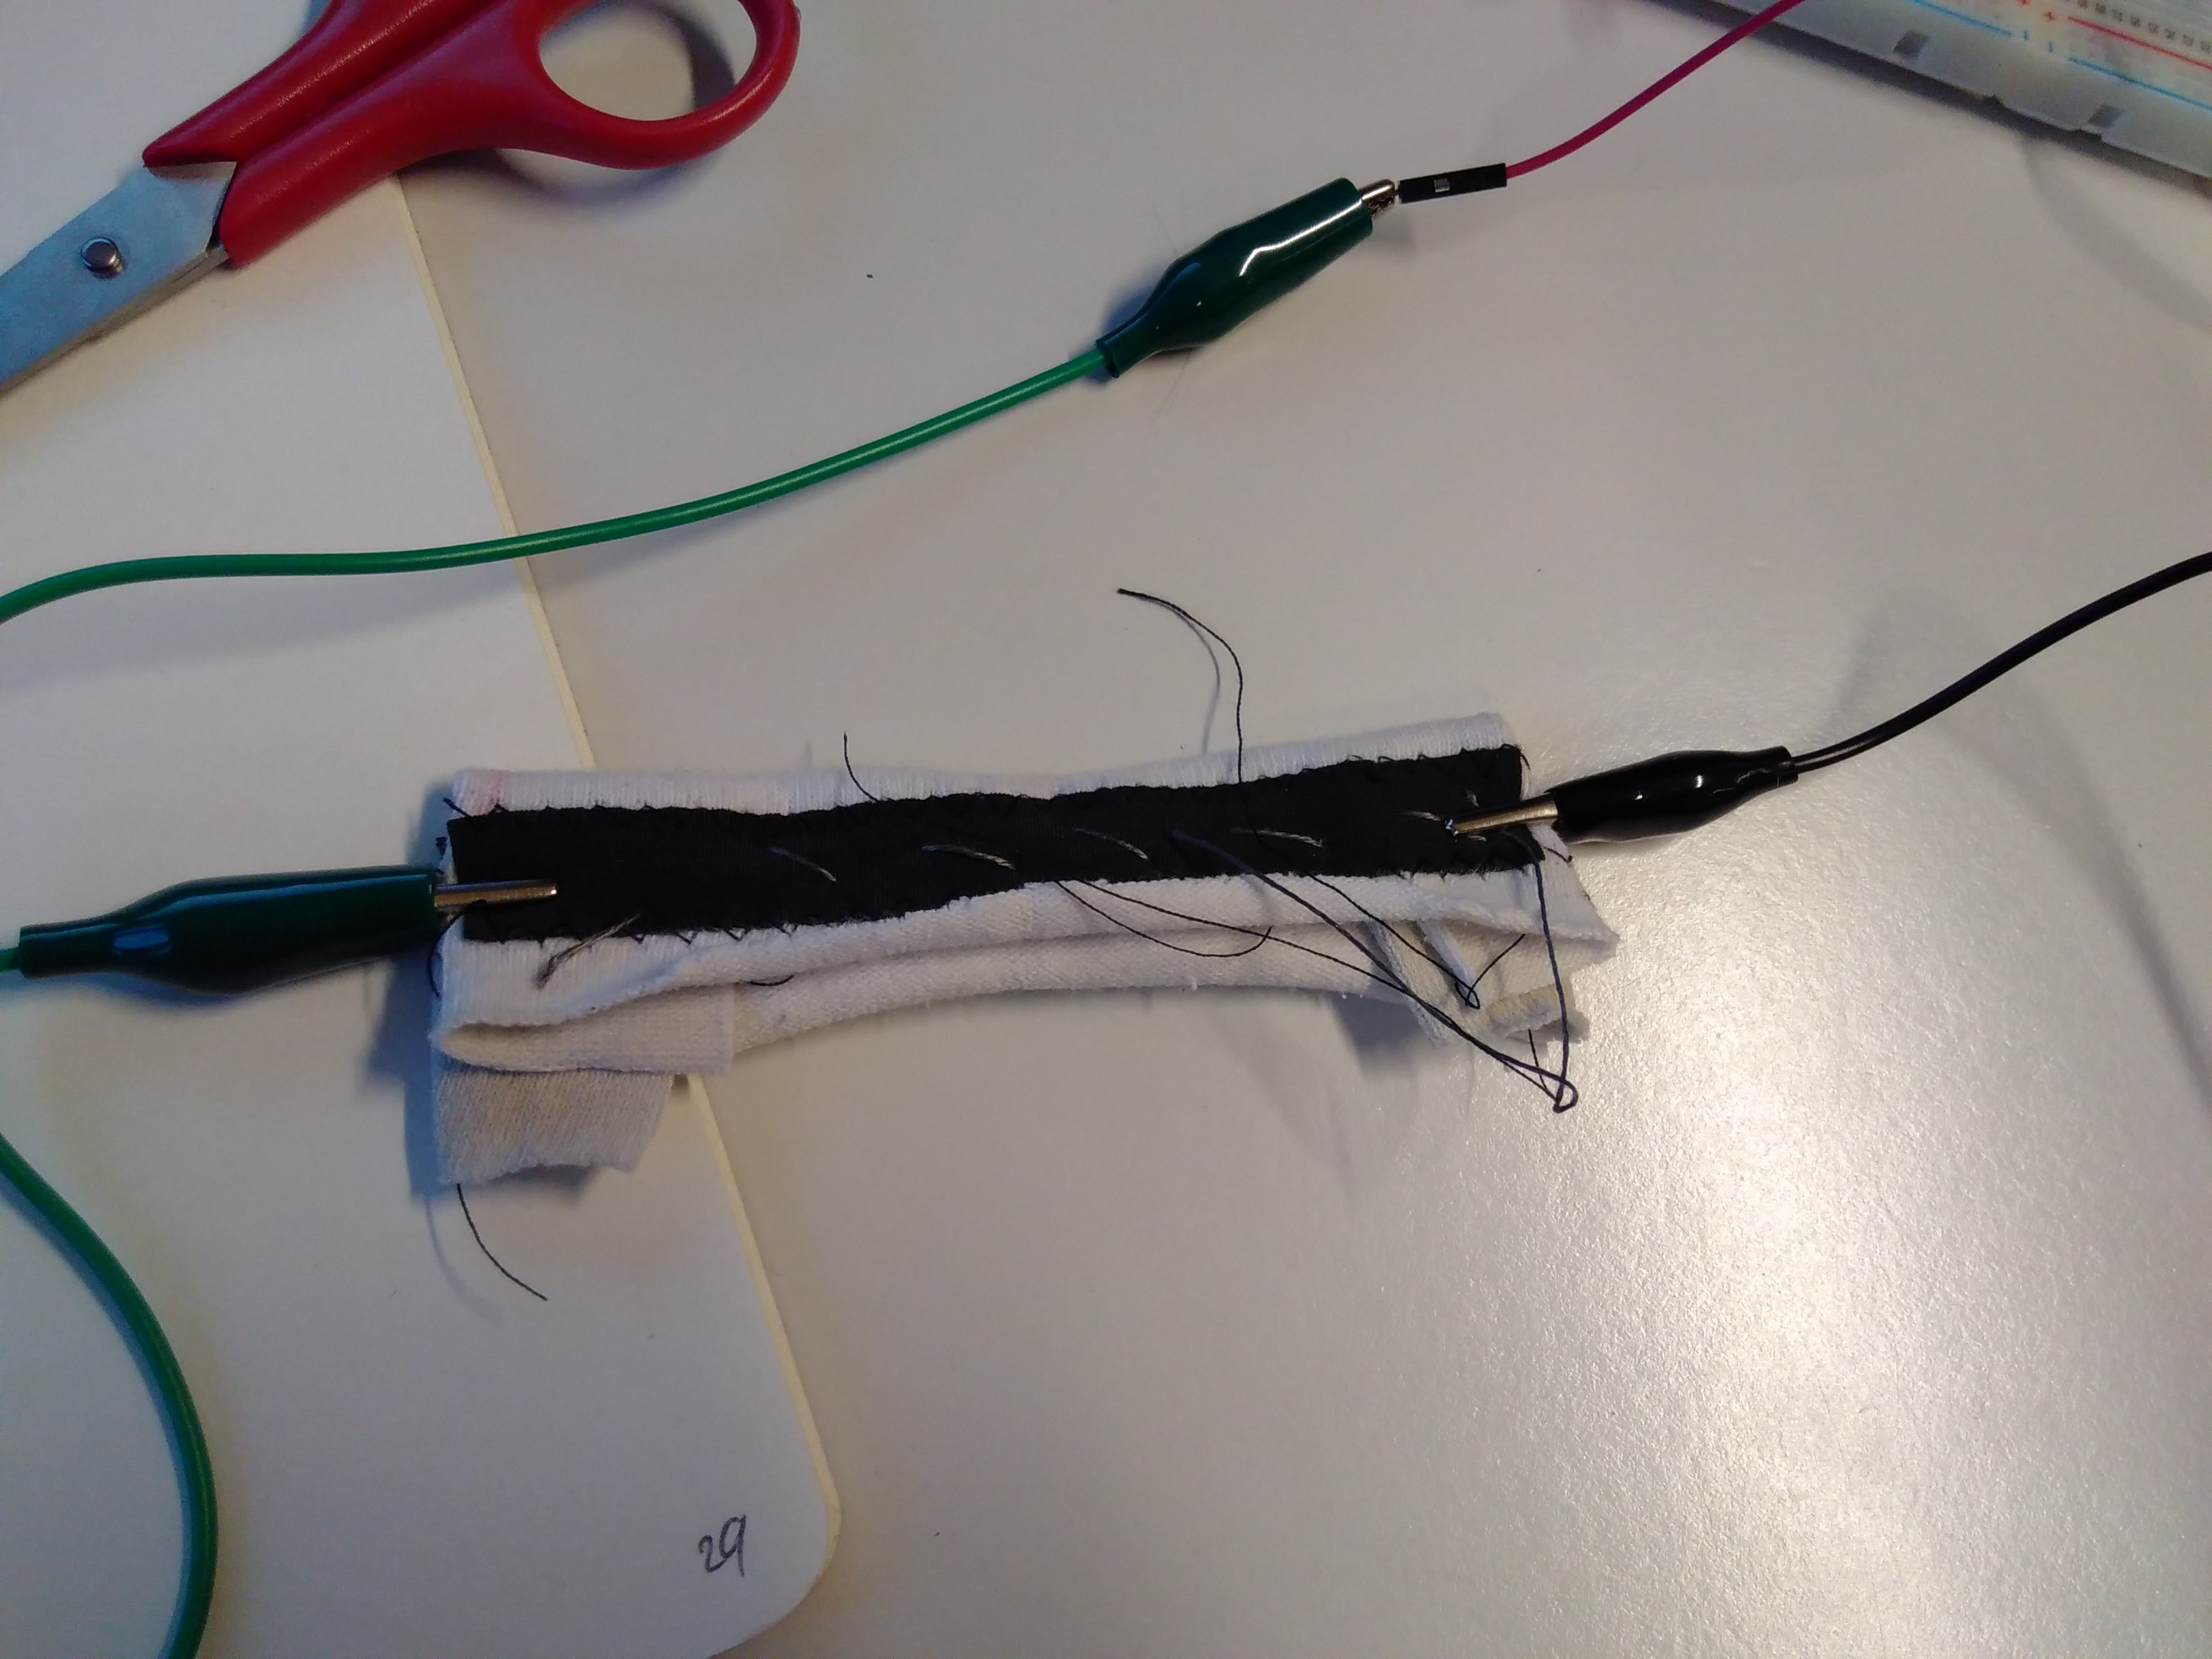
\includegraphics[width=0.47\textwidth]{images/HW/softsens_stretch.jpg}}\hfill
    \caption{Examples of two soft sensors we experimented with} 
    \label{fig:softsens}
\end{figure}

\subsection{Hard <-> Soft interfaces}
In our first prototype, we used banana cables attached to safety pins to ensure connectivity of the textile pads to the microcontroller. The second prototype had crimp pins attached to the conductive threads. The third prototype (MS6) will probably have the conductive threads/textile tracks attached to the secondary PCB.

\subsubsection{Next steps} For China or the next semester, we would like to have a compact, robust and user-friendly connector. Such connector could be designed with pogo pins on one side (PCB or textile) and connecting pads on the opposite side to ensure proper connectivity in a user-friendly and compact packaging. This design has been inspired by the connectors for different modules found in the Fairphone (Fig. \ref{fig:fp}).

\begin{figure}[H]
    \centering
    \subfloat[Pogo pin connector\label{fig:fp_connector}]{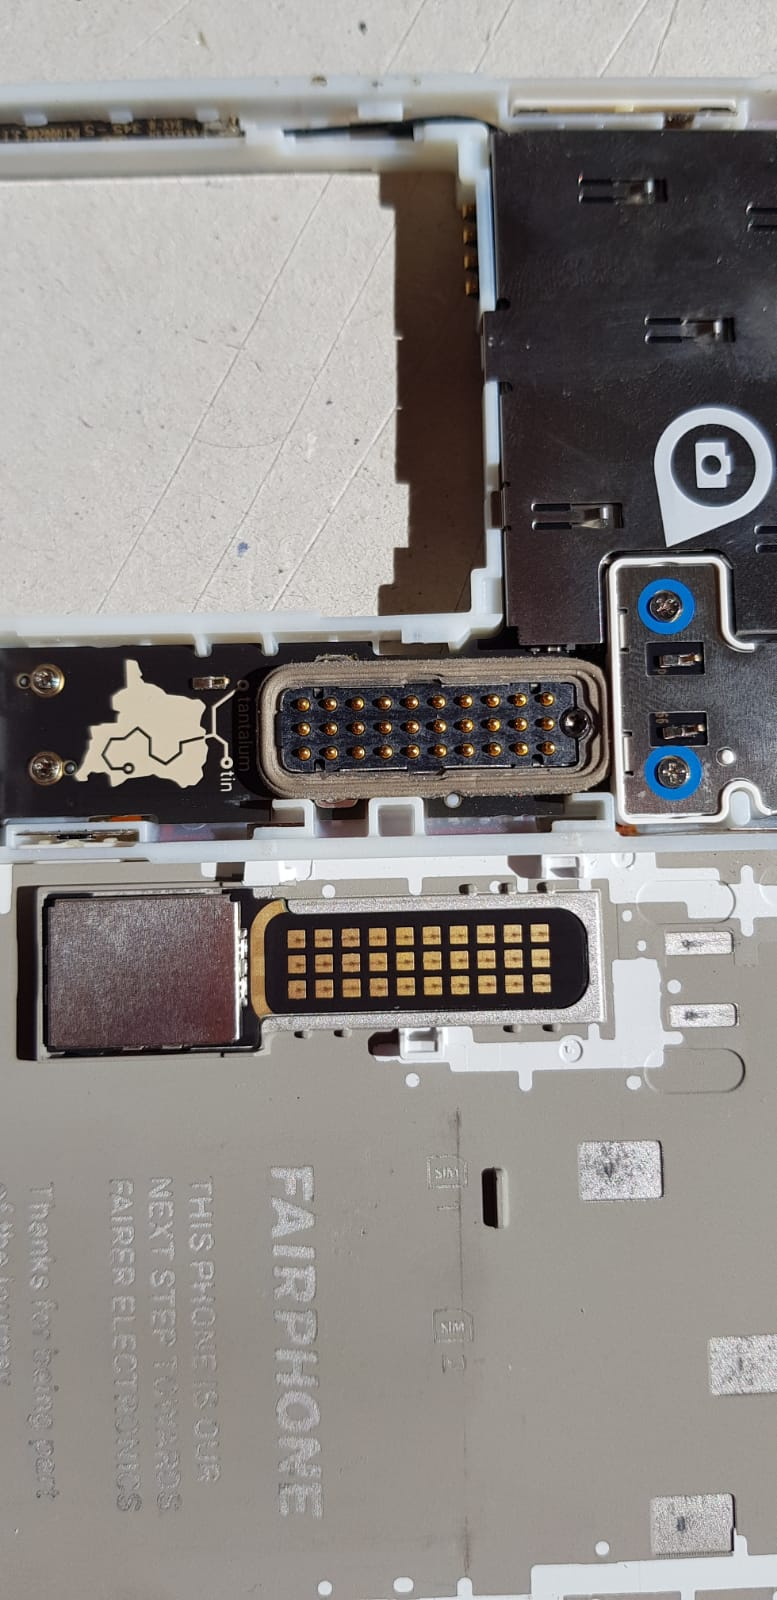
\includegraphics[width=0.47\textwidth]{images/HW/FP_connector.jpg}}\hfill
    \subfloat[Connector with LED element\label{fig:fp_LED}] {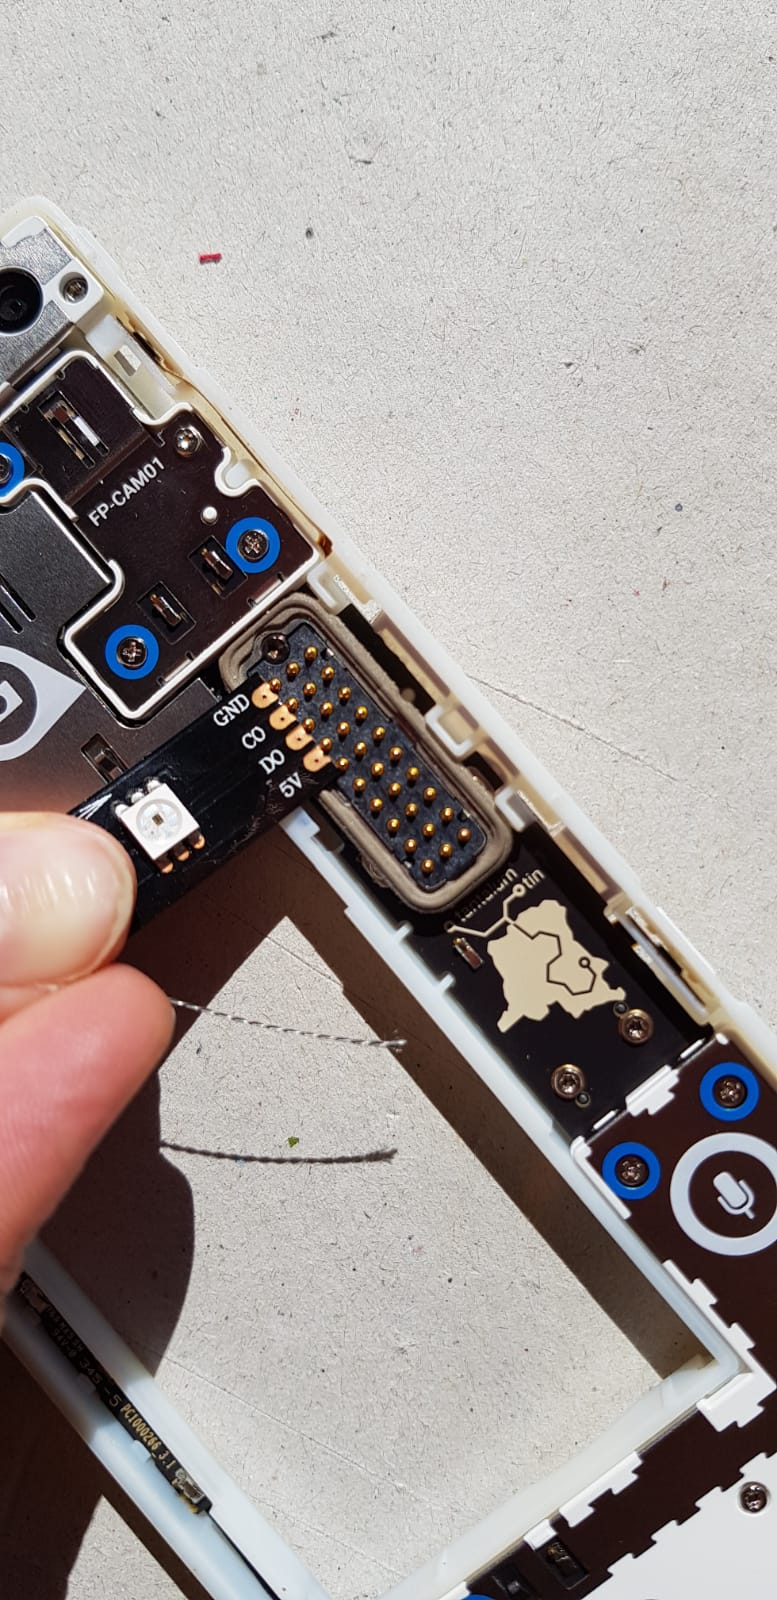
\includegraphics[width=0.47\textwidth]{images/HW/FP_connect_LED.jpg}}\hfill
    \caption{Example of pogo pin connector from Fairphone's electronics} 
    \label{fig:fp}
\end{figure}